%% Copyright (c) 2002, 2010 Sam Williams
%% Copyright (c) 2010 Richard M. Stallman
%% Copyright (c) 2014 Posts & Telecom Press
%% Permission is granted to copy, distribute and/or modify this
%% document under the terms of the GNU Free Documentation License,
%% Version 1.3 or any later version published by the Free Software
%% Foundation; with no Invariant Sections, no Front-Cover Texts, and
%% no Back-Cover Texts. A copy of the license is included in the
%% file called ``gfdl.tex''.
\chapter{\ifdefined\eng
A Portrait of the Hacker as a Young Man
\fi
\ifdefined\chs
黑客正年少
\fi}
\ifdefined\eng
\chaptermark{A Portrait of the Hacker}
\fi
\thispagestyle{empty}
\ifdefined\eng
Richard Stallman's mother, Alice Lippman, still remembers the moment she realized her son had a special gift.
\fi

\ifdefined\chs
理查德·斯托曼的母亲,爱丽丝·李普曼(Alice Lippman)始终还记得她意识到斯托曼天赋的那一刻。
\fi

\ifdefined\eng
``I think it was when he was eight,'' Lippman recalls.
\fi

\ifdefined\chs
``我记得他那会才八岁。''李普曼回忆着。
\fi

\ifdefined\eng
%% v1v2 s
The year was 1961, and Lippman, a recently divorced single mother, was \ifdefined\vone wiling \fi\ifdefined\vtwo whiling \fi away a weekend afternoon within the family's tiny one-bedroom apartment on Manhattan's Upper West Side. Leafing through a copy of Scientific American, Lippman came upon her favorite section, the Martin Gardner-authored column titled ``Mathematical Games.'' A substitute art teacher, Lippman always enjoyed Gardner's column for the brain-teasers it provided. With her son already ensconced in a book on the nearby sofa, Lippman decided to take a crack at solving the week's feature puzzle.
\fi

\ifdefined\chs
那是1961年,李普曼刚刚离异,做了单身妈妈。她家位于曼哈顿上西城,是一个一居室的小公寓。一个周末下午,她正在自己家里翻着一期《科学美国人》杂志,打发时光。她翻开自己最喜欢的一版,马丁⋅加德纳(Martin Gardner)主编的专栏:《数学游戏》。李普曼一个教艺术的代课老师,常常被这一专栏的各种头脑游戏吸引。她看了一眼在旁边沙发上老老实实待着的儿子,决定开始挑战本周的思考题。
\fi

\ifdefined\eng
``I wasn't the best person when it came to solving the puzzles,'' she admits. ``But as an artist, I found they really helped me work through conceptual barriers.''
\fi

\ifdefined\chs
``其实,这些题目我做得不是很好,''李普曼坦言,``可作为艺术家,我发现它们可以帮我缓解压力,激发灵感。''
\fi

\ifdefined\eng
Lippman says her attempt to solve the puzzle met an immediate brick wall. About to throw the magazine down in disgust, Lippman was surprised by a gentle tug on her shirt sleeve.
\fi

\ifdefined\chs
可她刚一开始做,就遇到了障碍。眼看她就打算扔开杂志,放弃解答了,可这时候,她发现有人正在轻拽她的衣袖。
\fi

\ifdefined\eng
``It was Richard,'' she recalls, ``He wanted to know if I needed any help.''
\fi

\ifdefined\chs
``那是理查德,''她回忆道,``他想问我要不要帮忙。''
\fi

\ifdefined\eng
Looking back and forth, between the puzzle and her son, Lippman says she initially regarded the offer with skepticism. ``I asked Richard if he'd read the magazine,'' she says. ``He told me that, yes, he had and what's more he'd already solved the puzzle. The next thing I know, he starts explaining to me how to solve it.''
\fi

\ifdefined\chs
她看看自己儿子,又回过头看看杂志上的题目,她还是有点半信半疑。``我问理查德,你读过这杂志了?''李普曼说,``理查德说读过了。而且他竟然已经解决这个题目了。之后,我就记得他开始给我讲解答题思路。''
\fi

\ifdefined\eng
Hearing the logic of her son's approach, Lippman's skepticism quickly gave way to incredulity. ``I mean, I always knew he was a bright boy,'' she says, ``but this was the first time I'd seen anything that suggested how advanced he really was.''
\fi

\ifdefined\chs
听着自己儿子清晰的逻辑,李普曼开始的半信半疑瞬间转变,一切让她觉得难以置信。``我知道理查德很聪明,''她说,``可这次却是实实在在让我见识了他究竟有多聪明。''
\fi

\ifdefined\eng
Thirty years after the fact, Lippman punctuates the memory with a laugh. ``To tell you the truth, I don't think I ever figured out how to solve that puzzle,'' she says. ``All I remember is being amazed he knew the answer.''
\fi

\ifdefined\chs
三十几年过去了,李普曼回忆起这事,最后笑道,``老实说,我到现在都没明白那道题是怎么做的。我能记得的,只是当时非常震惊,感叹理查德居然能做出那个题目。''
\fi

\ifdefined\eng
Seated at the dining-room table of her second Manhattan apartment -- the same spacious three-bedroom complex she and her son moved to following her 1967 marriage to Maurice Lippman, now deceased -- Alice Lippman exudes a Jewish mother's mixture of pride and bemusement when recalling her son's early years. The nearby dining-room credenza offers an eight-by-ten photo of Stallman glowering in full beard and doctoral robes. The image dwarfs accompanying photos of Lippman's nieces and nephews, but before a visitor can make too much of it, Lippman makes sure to balance its prominent placement with an ironic wisecrack.
\fi

\ifdefined\chs
李普曼坐在餐桌前,这里是她在曼哈顿住过的第二个公寓,在一座公寓楼里,是一个三居室的宽敞房子。1967年,她再婚嫁给了莫里斯·李普曼(Maurice Lippman),就带着斯托曼搬到了这所公寓里。时过境迁,莫里斯已经去世,斯托曼也长大成人。谈起当年抚养斯托曼,这位犹太妈妈流露出的尽是自豪和欣慰。在餐厅的橱柜里,摆放着一张8英寸*10英寸的照片。照片里是满脸络腮胡须的斯托曼,身穿博士服。这张照片摆在那里,让其他几张李普曼侄子侄女的照片显得不再引人注意。不过在客人问起这张照片之前,李普曼总会先调侃几句,解释一下为什么把它放到这么显眼的地方。
\fi

\ifdefined\eng
``Richard insisted I have it after he received his honorary doctorate at the University of Glasgow,'' says Lippman. ``He said to me, `Guess what, mom? It's the first graduation I ever attended.'\hspace{0.01in}''\ifdefined\vone\endnote{See Michael Gross, ``Richard Stallman: High School Misfit, Symbol of Free Software, MacArthur-certified Genius'' (1999). This interview is one of the most candid Stallman interviews on the record. I recommend it highly. \url{http://www.mgross.com/interviews/stallman1.html}}\fi\ifdefined\vtwo\endnote{One of the major background sources for this chapter was the interview ``Richard Stallman: High School Misfit, Symbol of Free Software, MacArthur-Certified Genius'' by Michael Gross, author of the 1999 book \textit{Talking About My Generation}, a collection of interviews with notable personalities from the so-called ``Baby Boom'' generation. Although Stallman did not make it into the book, Gross published the interview as an online supplement to the book's web site. The URL for the interview has changed several times since I first came across it. According to various readers who have gone searching for it, you can now find the interview at \url{http://www.mgross.com/MoreThgsChng/interviews/stallman1.html}.}\fi
\fi

\ifdefined\chs
``理查德坚持要把这张相片给我。这是他当年获得英国格拉斯哥大学(University of
Glasgow)荣誉博士学位的时候照的。他跟我说,`你看,这是我有生以来参加的第一个毕业典礼\ifdefined\vone\endnote{参见迈克尔⋅格劳斯(Michael Gross)1999年的访谈:Richard Stallman: High School Misfit, Symbol of Free Software, MacArthur-certified Genius,这篇访谈是我迄今为止看到过的有关斯托曼的最为中立的作品,向广大读者强烈推荐。\url{http://www.mgross.com/interviews/stallman1.html}}\fi\ifdefined\vtwo\endnote{本章内容的主要背景资料来源于Michael Gross的一篇采访《Richard Stallman: High School Misfit, Symbol of Free Software, MacArthur-Certified Genius》,Gross是1999年出版的《\textit{Talking About My Generation}》一书的作者,这本书中记录了很多对著名人士的访谈。虽然对于斯托曼的访谈最终没有收录到这本书中,但是Gross把它作为补充材料在发布在了这本书的网站上。这篇访谈的网址迁移过很多次,目前根据读者的反馈,你可以在这个地址读到这篇文章:\url{http://mgross.com/writing/books/the-more-things-change/bonus-chapters/richard-stallman-high-school-misfit-symbol-of-free-software-macarthur-certified-genius/}}\fi。'\hspace{0.01in}''
\fi

\ifdefined\eng
Such comments reflect the sense of humor that comes with raising a child prodigy. Make no mistake, for every story Lippman hears and reads about her son's stubbornness and unusual behavior, she can deliver at least a dozen in return.
\fi

\ifdefined\chs
抚养理查德·斯托曼这么一个孩子,李普曼总是有很多话可说。每当别人说起她儿子最新的各种或古怪或固执的行为时,她总会翻出更多类似陈年旧事作为回应。
\fi

\ifdefined\eng
``He used to be so conservative,'' she says, throwing up her hands in mock exasperation. ``We used to have the worst arguments right here at this table. I was part of the first group of public city school teachers that struck to form a union, and Richard was very angry with me. He saw unions as corrupt. He was also very opposed to social security. He thought people could make much more money investing it on their own. Who knew that within 10 years he would become so idealistic? All I remember is his stepsister coming to me and saying, `What is he going to be when he grows up? A fascist?'\hspace{0.01in}''\ifdefined\vtwo\endnote{RMS: I don't remember telling her this.  All I can say is I strongly disagree with those views now.  When I was in my teens, I lacked compassion for the difficulties most people encounter in life; my problems were different.  I did not appreciate how the wealthy will reduce most people to poverty unless we organize at all levels to stop them.  I did not understand how hard it is for most people to resist social pressure to do foolish things, such as spend all their money instead of saving, since I hardly even noticed the pressure myself. In addition, unions in the 60s, when they were very powerful, were sometimes arrogant or corrupt.  But they are much weaker today, and the result is that economic growth, when it occurs, benefits mainly the rich.}\fi
\fi

\ifdefined\chs
``他以前是十足的保守派,''她说着,把双臂铺开,以示强调,``曾经就在这张桌子前,我们俩人展开过一次很激烈的争论。我曾经是城市公立学校教师,其中,我是第一批坚持要成立工会的人。可理查德却觉得工会是腐败之源。他甚至非常反对社会保险。他认为,人们用买保险的钱,完全可以投资其他东西,赚更多的钱。当初谁会想到他十年之后会成为一个如此的理想主义者。我就记得当初我女儿曾问过我,`你说以后理查德长大了会是什么样?法西斯极右翼分子?'\hspace{0.01in}''
%\ifdefined\vtwo\endnote{RMS:我不记得我跟她说过这些。我只能说我现在很不赞同这里描述的观点。在我十几岁时,我遇到的问题跟其他同龄人并不相同。}\fi
\fi

\ifdefined\eng
As a single parent for nearly a decade -- she and Richard's father, Daniel Stallman, were married in 1948, divorced in 1958, and split custody of their son afterwards -- Lippman can attest to her son's aversion to authority. She can also attest to her son's lust for knowledge. It was during the times when the two forces intertwined, Lippman says, that she and her son experienced their biggest battles.
\fi

\ifdefined\chs
李普曼1948年和理查德的父亲丹尼尔·斯托曼(Daniel Stallman)结婚,于1958年离异。李普曼成了单身妈妈,抚养和监护这孩子的重担几乎都压在了她的身上。一路走来,她见证了她这个儿子蔑视权威的个性,更见证了他对知识的如饥似渴。这两股力量在她儿子身上几经纠缠,也让李普曼和理查德·斯托曼有过不少摩擦冲突。
\fi

\ifdefined\eng
``It was like he never wanted to eat,'' says Lippman, recalling the behavior pattern that set in around age eight and didn't let up until her son's high-school graduation in 1970. ``I'd call him for dinner, and he'd never hear me. I'd have to call him 9 or 10 times just to get his attention. He was totally immersed.''
\fi

\ifdefined\chs
``他好像一直都不想吃饭一样,''李普曼回忆着儿子八岁到1970年中学毕业的那段时间,``他就跟个聋子似的,我每次都得叫他九到十次,他才肯过来吃饭。''
\fi

\ifdefined\eng
Stallman, for his part, remembers things in a similar fashion, albeit with a political twist.
\fi

\ifdefined\chs
同样是这件事,到了斯托曼嘴里,就掺进了政治的意味。
\fi

\ifdefined\eng
``I enjoyed reading,'' he says. ``If I wanted to read, and my mother told me to go to the kitchen and eat or go to sleep, I wasn't going to listen. I saw no reason why I couldn't read. No reason why she should be able to tell me what to do, period. Essentially, what I had read about, ideas such as democracy and individual freedom, I applied to myself. I didn't see any reason to exclude children from these principles.''
\fi

\ifdefined\chs
``我特别喜欢读书,''斯托曼说,``赶在我想读书的时候,我妈妈恰巧叫我去吃饭,我肯定不会去。我就觉得,凭什么我不能读书?凭什么我妈妈可以指点我该做什么,该读什么书。我坚持民主和个人自由。很多原则不应该仅仅局限在成人身上,未成年人也同样适用。''
\fi

\ifdefined\eng
The belief in individual freedom over arbitrary authority extended to school as well. Two years ahead of his classmates by age 11, Stallman endured all the usual frustrations of a gifted public-school student. It wasn't long after the puzzle incident that his mother attended the first in what would become a long string of parent-teacher conferences.
\fi

\ifdefined\chs
斯托曼坚信个人自由高于任何权威。这样的思想也被他带到了校园之中。斯托曼比其他的孩子入学早了两年。和很多天才儿童一样,斯托曼也有着自己的烦恼。那次他帮妈妈解决完杂志上的数学题之后没多久,老师就把妈妈约去学校,进行了一次长谈。
\fi

\ifdefined\eng
%% v1v2 s fixed
``He absolutely refused to write papers,'' says Lippman, recalling an early controversy. ``I think the last paper he wrote before his senior year in high school was an essay on the history of the number system in the west for a fourth-grade teacher.''
\fi

\ifdefined\chs
``他拒绝写作文、写文章,''李普曼回忆着当时的情景,``除了高中最后一年,他最后一次写作文是在四年级的时候。那是一篇关于西方计数系统的文章。''
\fi

\ifdefined\eng
Gifted in anything that required analytical thinking, Stallman gravitated toward math and science at the expense of his other studies. What some teachers saw as single-mindedness, however, Lippman saw as impatience. Math and science offered simply too much opportunity to learn, especially in comparison to subjects and pursuits for which her son seemed less naturally inclined. Around age 10 or 11, when the boys in Stallman's class began playing a regular game of touch football, she remembers her son coming home in a rage. ``He wanted to play so badly, but he just didn't have the coordination skills,'' Lippman recalls. ``It made him so angry.''
\fi

\ifdefined\chs
凭借着分析性思维的天赋,斯托曼沉浸在数理化的世界,而代价则是其他方面严重欠缺。老师们看来是头脑简单的行为,在李普曼看来,倒觉得是斯托曼好强所致。比起其他斯托曼天生就不太在行的领域来说,数学和自然科学给斯托曼提供了太多的学习机会。大概在10~11岁那年,斯托曼的同学们都在玩触式橄榄球。她记得有一次斯托曼回家特别生气。``他当时非常想和他们一起玩,可他身体的协调性实在太差了,''李普曼回忆道,``这实在让他非常恼火。''
\fi

\ifdefined\eng
The anger eventually drove her son to focus on math and science all the more. Even in the realm of science, however, her son's impatience could be problematic. Poring through calculus textbooks by age seven, Stallman saw little need to dumb down his discourse for adults. Sometime, during his middle-school years, Lippman hired a student from nearby Columbia University to play big brother to her son. The student left the family's apartment after the first session and never came back. ``I think what Richard was talking about went over his head,'' Lippman speculates.
\fi

\ifdefined\chs
这份感觉让斯托曼更埋头在理科世界里。可哪怕在数理化的世界,他的好强有时也会成问题。在八岁的时候,斯托曼就已经把微积分教材翻了个透。他觉得自己完全没必要在大人面前装成傻傻的天真宝宝。他中学的时候,妈妈曾从附近的哥伦比亚大学里雇来了一位大学生,以期在斯托曼面前扮演大哥哥的角色。结果这位学生来了一次就没再来了。``我觉得斯托曼当时讨论的问题可能超出他的极限了。''李普曼推测。
\fi

\ifdefined\eng
%% v1v2 s
Another favorite maternal anecdote dates back to the early 1960s, shortly after the puzzle incident. Around age seven, two years after the divorce and relocation from Queens, Richard took up the hobby of launching model rockets in nearby Riverside Drive Park. What started as aimless fun soon took on an earnest edge as her son began recording the data from each launch. Like the interest in mathematical games, the pursuit drew little attention until one day, just before a major NASA launch, Lippman checked in on her son to see if he wanted to watch.
\fi

\ifdefined\chs
另一个李普曼喜欢提起的小事,发生在20世纪60年代早期。那时,李普曼已经离异两年,也从皇后区搬了出来。斯托曼当时七岁,迷上了火箭模型。他常常去河滨公园发射火箭模型。一开始他只是随便瞎玩,可后来他开始记录每次的发射数据。起初,这些行为并没引起李普曼注意,她觉得这个兴趣就和玩数学游戏一样。可有一次NASA(美国国家航空航天局)发射火箭前,李普曼问斯托曼要不要看电视上的现场直播。
\fi

\ifdefined\eng
%% v1v2 s fixed
``He was fuming,'' Lippman says. ``All he could say to me was, `But I'm not published yet.' Apparently he had something that he really wanted to show NASA.''
\fi

\ifdefined\chs
``他可逗了,上来就跟我说,`可我的研究成果还没发表呢!'就好像真有点资料要给NASA看似的。''
\fi

\ifdefined\eng
%% v1v2 s 
Such anecdotes offer early evidence of the intensity that would become Stallman's chief trademark throughout life. When other kids came to the table, Stallman stayed in his room and read. When other kids played Johnny Unitas, Stallman played Werner von Braun. ``I was weird,'' Stallman says, summing up his early years succinctly in a 1999 interview. ``After a certain age, the only friends I had were teachers.''\endnote{\textit{Ibid.}}%%  Stallman was not ashamed of his weird characteristics, distinguishing them from the social ineptness that he did regard as a failing.  However, both contributed together to his social exclusion.
\fi

\ifdefined\chs
这个小事倒很好地表现了斯托曼性格中独具一格的特点——紧迫感。这种紧迫感一直伴随在他左右。其他孩子还在桌前玩耍的时候,他在房间里读书;别的孩子在痴迷橄榄球运动员约翰尼⋅尤尼塔斯(Johnny Unitas)的时候,斯托曼则崇拜着火箭专家。``我当时就是这么古怪,''斯托曼在1999年接受一次采访的时候,如此总结着自己的童年,``没过几年,我的朋友就只剩下各位老师了\endnote{\textit{同上}}。'' %%对于他自己古怪的性格,斯托曼并不觉得丢人,但是他对于自己不擅长社交这一点总是深感遗憾。不过,正是他e特有性格和社交能力的缺乏造成了他与现实社会之间的隔阂。
\fi

\ifdefined\eng
Although it meant courting more run-ins at school, Lippman decided to indulge her son's passion. By age 12, Richard was attending science camps during the summer and private school during the school year. When a teacher recommended her son enroll in the Columbia Science Honors Program, a post-Sputnik program designed for gifted middle- and high-school students in New York City, Stallman added to his extracurriculars and was soon commuting uptown to the Columbia University campus on Saturdays.
\fi

\ifdefined\chs
虽然斯托曼总比同龄人显得古怪很多,但李普曼还是决定让他追求自己的兴趣和热情。12岁那年,斯托曼参加了科学夏令营,之后上了私立中学。学校的老师建议让斯托曼参加``哥伦比亚科学之星计划''。该计划旨在为具有天赋的纽约中学生提供更多的学习机会。斯托曼参加了这个计划,于是每周六,他都会赶去哥伦比亚大学。
\fi

\ifdefined\eng
Dan Chess, a fellow classmate in the Columbia Science Honors Program, recalls Richard Stallman seeming a bit weird even among the students who shared a similar lust for math and science. ``We were all geeks and nerds, but he was unusually poorly adjusted,'' recalls Chess, now a mathematics professor at Hunter College. ``He was also smart as shit. I've known a lot of smart people, but I think he was the smartest person I've ever known.''
\fi

\ifdefined\chs
%% Patch Pending
丹·柴斯(Dan Chess)也参加了科学之星计划,他回忆中的斯托曼,哪怕在众多同龄的科学爱好者之中,也算是古怪的。``我们都是书呆子、技术宅,可斯托曼在这圈子里仍是特立独行的''如今的柴斯已经是亨特学院数学系的教授,他回忆道,``他更是聪明绝顶。我见过很多聪明人,可斯托曼是我见过最棒的。''
\fi

\ifdefined\eng
Seth Breidbart, a fellow Columbia Science Honors Program alumnus, offers bolstering testimony. A computer programmer who has kept in touch with Stallman thanks to a shared passion for science fiction and science-fiction conventions, he recalls the 15-year-old, buzz-cut-wearing Stallman as ``scary,'' especially to a fellow 15-year-old.
\fi

\ifdefined\chs
另外一个科学之星计划的成员——赛思·布莱德巴特(Seth Breidbart),也提供了类似的证据。布莱德巴特如今也是个程序员,依然和斯托曼保持联系。他回忆当年只有15岁、剃了短发的斯托曼甚至有些``令人生畏''。
\fi

\ifdefined\eng
``It's hard to describe,'' Breidbart says. ``It wasn't like he was unapproachable. He was just very intense. [He was] very knowledgeable but also very hardheaded in some ways.''
\fi

\ifdefined\chs
``这可难解释了。不是说斯托曼会拒人千里,只是说,在他身上,总能看到一种紧迫感。他知识丰富,可有些地方又非常爱钻牛角尖,非常固执。''布莱德巴特回忆说。
\fi

\ifdefined\eng
%% v1v2 m
Such descriptions give rise to speculation: are judgment-laden adjectives like "intense" and "hardheaded" simply a way to describe traits that today might be categorized under juvenile behavioral disorder? A December, 2001, \textit{Wired} magazine article titled "The Geek Syndrome" paints the portrait of several scientifically gifted children diagnosed with high-functioning autism or Asperger Syndrome. In many ways, the parental recollections recorded in the Wired article are eerily similar to the ones offered by Lippman. Even Stallman has indulged in psychiatric revisionism from time to time. During a 2000 profile for the Toronto Star, Stallman described himself to an interviewer as ``borderline autistic,''\endnote{See Judy Steed, \textit{Toronto Star}, \textit{BUSINESS}, (October 9, 2000): C03.

\begin{quote}
His vision of free software and social cooperation stands in stark contrast to the isolated nature of his private life. A Glenn Gould-like eccentric, the Canadian pianist was similarly brilliant, articulate, and lonely. Stallman considers himself afflicted, to some degree, by autism: a condition that, he says, makes it difficult for him to interact with people.
\end{quote}
} a description that goes a long way toward explaining a lifelong tendency toward social and emotional isolation and the equally lifelong effort to overcome it.

\fi

\ifdefined\chs
``紧迫感''、``爱钻牛角尖''、``固执'',这样几个形容词放在一起,放在今天哪个中学生身上,多半会让人觉得是青春期综合症的症状。其实,在2001年12月的《连线》杂志中,就有一篇名为《天才综合症》的报道,采访了几个自闭症儿童患者,他们都在数学和科学方面具有天赋。报道中,患者家长对患者的描述,在很多方面都类似李普曼对斯托曼的形容。哪怕是斯托曼,提到自己精神方面,也曾犹豫再三。在一份2000年《多伦多之星》报纸上的资料中,斯托曼曾描述自己为``濒临自闭''\endnote{朱迪·丝蒂特(Judy Steed),《多伦多之星》,2000年10月9日,C03版。

\begin{quote}
他对自由软件和社会合作的愿景明显与他孤立的个人生活格格不入。他的古怪与加拿大钢琴家格连⋅古尔德(Glenn Gould)非常相似,他们都是非常聪明、善于表达的人,但是同时也都很孤独。斯托曼觉得自己在某种程度上被自闭症所折磨,他总是觉得自己与其他人打交道非常困难。
\end{quote}},以此解释自己一直以来在社交方面的孤僻,并介绍了自己如何不断克服这种心理。
\fi

\ifdefined\eng
%% v1v2 m
Such speculation benefits from the fast and loose nature of most so-called ``behavioral disorders'' nowadays, of course. As Steve Silberman, author of ``The Geek Syndrome,'' notes, American psychiatrists have only recently come to accept Asperger Syndrome as a valid umbrella term covering a wide set of behavioral traits. The traits range from poor motor skills and poor socialization to high intelligence and an almost obsessive affinity for numbers, computers, and ordered systems.\endnote{See Steve Silberman, ``The Geek Syndrome,'' \textit{Wired} (December, 2001), \url{http://www.wired.com/wired/archive/9.12/aspergers_pr.html}.} Reflecting on the broad nature of this umbrella, Stallman says its possible that, if born 40 years later, he might have merited just such a diagnosis. Then again, so would many of his computer-world colleagues.
\fi

\ifdefined\chs
这种判断和当下流行的``异常行为''研究是分不开的。《天才综合症》的作者史蒂夫·西尔贝曼(Steve Silberman)介绍,美国的心理学家在近年来才把自闭症作为一系列症状行为特征的统称。这些行为包括:不擅运动,不擅社交,但又对数学,计算机和类似的具有规律的系统有着极度的依恋,并擅长于此\endnote{史蒂夫·西尔贝曼,《天才综合症》,《\textit{连线}》2001年12月刊。\url{http://www.wired.com/wired/archive/9.12/aspergers_pr.html}}。在自闭症这样一个统称之下,理查德坦言,要是出生在当下,很可能就被拉去做检查了。当然,他的那群在计算机世界中的朋友,也一样跑不了。
\fi

\ifdefined\eng
%% v1v2 s fixed
``It's possible I could have had something like that,'' he says. ``On the other hand, one of the aspects of that syndrome is difficulty following rhythms. I can dance. In fact, I love following the most complicated rhythms. It's not clear cut enough to know.''  %%Another possibility is that Stallman had a ``shadow syndrome'' which goes some way in the direction of Asperger's syndrome but without going beyond the limits of normality.\endnote{See John Ratey and Catherine Johnson, ``Shadow Syndromes.''}
\fi

\ifdefined\chs
``我当初也许还真有这种毛病吧,''斯托曼说,``可自闭症患者的另一个症状是对音乐和节奏迟钝。我还能跳舞呢,而且我对节奏特别敏感,喜欢复杂的节奏。这么看倒也未必是自闭症了。''%%\endnote{参考John Ratey与Catherine Johnson,``Shadow Syndromes''。}
\fi

\ifdefined\eng
Chess, for one, rejects such attempts at back-diagnosis. ``I never thought of him [as] having that sort of thing,'' he says. ``He was just very unsocialized, but then, we all were.''
\fi

\ifdefined\chs
柴斯则非常反对这种推断:``我从不觉得斯托曼有自闭症。他当初就是社交方面有点障碍,可我们这群人都这样。''
\fi

\ifdefined\eng
Lippman, on the other hand, entertains the possibility. She recalls a few stories from her son's infancy, however, that provide fodder for speculation. A prominent symptom of autism is an oversensitivity to noises and colors, and Lippman recalls two anecdotes that stand out in this regard. ``When Richard was an infant, we'd take him to the beach,'' she says. ``He would start screaming two or three blocks before we reached the surf. It wasn't until the third time that we figured out what was going on: the sound of the surf was hurting his ears.'' She also recalls a similar screaming reaction in relation to color: ``My mother had bright red hair, and every time she'd stoop down to pick him up, he'd let out a wail.''
\fi

\ifdefined\chs
而李普曼则认为确有此事。她说了斯托曼婴儿时期的一些事情,佐证这个结论。自闭症患者的一个显著症状,就是对噪声和颜色异常敏感。李普曼记起了两个事情:``当时斯托曼还是个婴儿,我们带他去海边,每次去,在离海有两三个街区的时候,他就开始大哭。去了三次,我们才发现,原来是他觉得海浪的声音太吵了,''接着,她又说了斯托曼当时对颜色的反应,``斯托曼姥姥的头发是亮红色的,每次他姥姥抱起他的时候,他也会大哭大叫。''
\fi

\ifdefined\eng
In recent years, Lippman says she has taken to reading books about autism and believes that such episodes were more than coincidental. ``I do feel that Richard had some of the qualities of an autistic child,'' she says. ``I regret that so little was known about autism back then.''
\fi

\ifdefined\chs
这几年,李普曼读了一些关于自闭症的书。她觉得斯托曼的这些行为绝非巧合:``我确实觉得理查德当时有很多自闭症儿童的症状。我真后悔当初对这种病没什么了解。''
\fi

\ifdefined\eng
Over time, however, Lippman says her son learned to adjust. By age seven, she says, her son had become fond of standing at the front window of subway trains, mapping out and memorizing the labyrinthian system of railroad tracks underneath the city. It was a hobby that relied on an ability to accommodate the loud noises that accompanied each train ride. ``Only the initial noise seemed to bother him,'' says Lippman. ``It was as if he got shocked by the sound but his nerves learned how to make the adjustment.''
\fi

\ifdefined\chs
李普曼说,时间一久,斯托曼也逐渐开始适应了环境。七岁的时候,他开始喜欢坐在地铁的第一节车厢里,透过司机窗口看着地铁隧道,记下地铁的路线。这必须得习惯了地铁的噪音才行。``只有启动时候的噪音会让他不安,''李普曼说,``一启动,他就跟被谁打了一下似的。不过他后来也逐渐习惯了。''
\fi

\ifdefined\eng
For the most part, Lippman recalls her son exhibiting the excitement, energy, and social skills of any normal boy. It wasn't until after a series of traumatic events battered the Stallman household, she says, that her son became introverted and emotionally distant.
\fi

\ifdefined\chs
李普曼回忆,斯托曼以前也和其他孩子一样,活泼快乐有生气。可家中一系列的变故,让他越来越内向,逐渐与人疏远。
\fi

\ifdefined\eng
The first traumatic event was the divorce of Alice and Daniel Stallman, Richard's father. Although Lippman says both she and her ex-husband tried to prepare their son for the blow, she says the blow was devastating nonetheless. ``He sort of didn't pay attention when we first told him what was happening,'' Lippman recalls. ``But the reality smacked him in the face when he and I moved into a new apartment. The first thing he said was, `Where's Dad's furniture?'\hspace{0.01in}''
\fi

\ifdefined\chs
第一件事就是斯托曼的父母离异。李普曼和斯托曼的父亲——丹尼尔⋅斯托曼,都有所准备,打算慢慢把离异的事实告诉斯托曼,希望不要对他产生太大影响。可结果依旧让斯托曼改变很多。李普曼回忆:``他一开始好像还没把这件事放在心上,可当我和他一起搬到新公寓的时候,他彻底意识到发生了什么。他的第一反应是,`爸爸的那些家具哪去了?'\hspace{0.01in}''
\fi

\ifdefined\eng
For the next decade, Stallman would spend his weekdays at his mother's apartment in Manhattan and his weekends at his father's home in Queens. The shuttling back and forth gave him a chance to study a pair of contrasting parenting styles that, to this day, leaves Stallman firmly opposed to the idea of raising children himself. Speaking about his father, a World War II vet who \ifdefined\vone passed away \fi\ifdefined\vtwo died \fi in early 2001, Stallman balances respect with anger. On one hand, there is the man whose moral commitment led him to learn French just so he could be more helpful to Allies when they'd \ifdefined\vone finally come. \fi\ifdefined\vtwo finally fight the Nazis in France. \fi On the other hand, there was the parent who always knew how to craft a put-down for cruel effect.\endnote{Regrettably, I did not get a chance to interview Daniel Stallman for this book. During the early research for this book, Stallman informed me that his father suffered from Alzheimer's. When I resumed research in late 2001, I learned, sadly, that Daniel Stallman had died earlier in the year.}
\fi

\ifdefined\chs
在接下来的十年,每周工作日,斯托曼都住在母亲的公寓;休息日则要跑去皇后区,在爸爸家里住。辗转之间,他也见识了两种完全不同的抚养方式。这一切,让他从此决定不会自己抚养小孩。理查德⋅斯托曼的父亲曾是参与过第二次世界大战的一名退伍老兵,于2001年去世。每当说起他,理查德⋅斯托曼总是对他又尊敬又恼火。一方面,这是一位有担当的士兵,他曾为了更好地帮助盟友,特地学习法语;另一方面,他又是个总会把事情变得残酷不堪的父亲\endnote{很遗憾,我最终没能采访到丹尼尔·斯托曼。本书写作之初,理查德·斯托曼曾告诉我他父亲患上了老年痴呆症。2001年,我继续写本书的时候,得知丹尼尔·斯托曼已经去世了。}。
\fi

\ifdefined\eng
``My father had a horrible temper,'' Stallman says. ``He never screamed, but he always found a way to criticize you in a cold, designed-to-crush way.''
\fi

\ifdefined\chs
%% TODO Patch Pending
``我爸爸脾气很坏''斯托曼说,``他虽然从不大吼大叫,但总能用一种冷嘲热讽的方式去批评指责你。''
%%``我爸爸脾气很坏。''斯托曼说,``他虽然从不大吼大叫,但总能用一种冷嘲热讽的方式,去批评指责你。''
\fi

\ifdefined\eng
As for life in his mother's apartment, Stallman is less equivocal. ``That was war,'' he says. ``I used to say in my misery, `I want to go home,' meaning to the nonexistent place that I'll never have.''
\fi

\ifdefined\chs
至于说起和母亲住在一起的日子,斯托曼的评价就不再那么模棱两可了:``我们俩之间可是战事频发。我常带着几分悲伤说`我想家了',其实我的意思是,所谓的`家'对我来说就是个幻想中的空中楼阁。''
\fi

\ifdefined\eng
%% v1v2 s
For the first few years after the divorce, Stallman found the tranquility that eluded him in the home of his paternal grandparents. Then, around age 10 his grandparents passed away in short succession. For Stallman, the loss was devastating. "I used to go and visit and feel I was in a loving, gentle environment," Stallman recalls. "It was the only place I ever found one, until I went away to college."
%%For the first few years after the divorce, Stallman found the tranquility that eluded him in the home of his paternal grandparents. One died when he was 8, and the other when he was 10. For Stallman, the loss was devastating. ``I used to go and visit and feel I was in a loving, gentle environment,'' Stallman recalls. ``It was the only place I ever found one, until I went away to college.''
\fi

\ifdefined\chs
父母离异后的最初几年,斯托曼还可以把祖父母和外祖父母家当作一个避风港。可在他10岁左右的时候,几位老人相继去世,斯托曼因此受到了巨大的打击。``以前还能去爷爷奶奶或者姥姥老爷家,能觉得有人疼我,有人爱我。上大学之前,那是唯一一个让我觉得如此温暖的地方。''
\fi

\ifdefined\eng
Lippman lists the death of Richard's paternal grandparents as the second traumatic event. ``It really upset him,'' she says. He was very close to both his grandparents. Before they died, he was very outgoing, almost a leader-of-the-pack type with the other kids. After they died, he became much more emotionally withdrawn.
\fi

\ifdefined\chs
李普曼把祖父母和外祖父母的去世列为第二个沉重打击斯托曼的家庭变故。``他当时悲痛欲绝。他和几位老人关系特别好,老人们去世之前,理查德特别开朗外向,都属于远近一带的`孩子王'的角色。他们一走,理查德一下子变得极度消沉。''
\fi

\ifdefined\eng
From Stallman's perspective, the emotional withdrawal was merely an attempt to deal with the agony of adolescence. Labeling his teenage years a ``pure horror,'' Stallman says he often felt like a deaf person amid a crowd of chattering music listeners.
\fi

\ifdefined\chs
对于斯托曼来讲,这种消沉则是一种躲避悲痛的行为。他把自己的青少年时期形容为``不寒而栗''。他说,就好比一个聋子,被扔到了一群音乐爱好者中间,眼睁睁看着他们聚在一起,谈音论乐。
\fi

\ifdefined\eng
%% v1v2 s
"I often had the feeling that I couldn't understand what other people were saying," says Stallman, recalling the emotional bubble that insulated him from the rest of the adolescent and adult world. "I could understand the words, but something was going on underneath the conversations that I didn't understand. I couldn't understand why people were interested in the things other people said."

%%``I often had the feeling that I couldn't understand what other people were saying,'' says Stallman, recalling his sense of exclusion. ``I could understand the words, but something was going on underneath the conversations that I didn't understand. I couldn't understand why people were interested in the things other people said.''
\fi

\ifdefined\chs
``我总有一种感觉,觉得无法理解周围人在说什么,''斯托曼回忆当初,说着自己如何被悲痛感包围以至无法与外界沟通,``我明白他们说的每个词,可总觉得在谈话背后,隐藏着我无法理解的东西。我不能理解别人为什么对旁人的话题如此感兴趣。''
\fi

\ifdefined\eng
%% v1v2 s
For all the agony it produced, adolescence would have a encouraging effect on Stallman's sense of individuality. At a time when most of his classmates were growing their hair out, Stallman preferred to keep his short. At a time when the whole teenage world was listening to rock and roll, Stallman preferred classical music. A devoted fan of science fiction, Mad magazine, and late-night TV, Stallman cultivated a distinctly off-the-wall personality that fed off the incomprehension of parents and peers alike.
%%For all the agony it produced, adolescence would have an encouraging effect on Stallman's sense of individuality. At a time when most of his classmates were growing their hair out, Stallman preferred to keep his short. At a time when the whole teenage world was listening to rock and roll, Stallman preferred classical music. A devoted fan of science fiction, \textit{Mad} magazine, and late-night TV, Stallman came to have a distinctly off-the-wall personality that met with the incomprehension of parents and peers alike.
\fi

\ifdefined\chs
悲伤往往会唤起青少年极度的自我意识,会强烈展示自己的个性和与众不同。那会儿,别的孩子都喜欢把头发留长,斯托曼则一头短发;全部青少年都开始迷恋摇滚乐,斯托曼则钟情于古典乐。他热衷科幻小说,喜欢读\textit{Mad}杂志,爱看深夜电视节目。他发展出了这种特立独行的个性,以此回避与这个世界的格格不入。
\fi

\ifdefined\eng
``Oh, the puns,'' says Lippman, still exasperated by the memory of her son's teenage personality. ``There wasn't a thing you could say at the dinner table that he couldn't throw back at you as a pun.''
\fi

\ifdefined\chs
李普曼回忆起斯托曼少年时的个性:``开玩笑,俏皮话,双关语。只要你在桌上抛出一句话,他肯定能借此抖个包袱、耍个宝。''
\fi

\ifdefined\eng
\ifdefined\vone
Outside the home, Stallman saved the jokes for the adults who tended to indulge his gifted nature. One of the first was a summer-camp counselor who handed Stallman a print-out manual for the IBM 7094 computer during his 12th year. To a preteenager fascinated with numbers and science, the gift was a godsend.\endnote{Stallman, an atheist, would probably quibble with this description. Suffice it to say, it was something Stallman welcomed. See previous note 1: ``As soon as I heard about computers, I wanted to see one and play with one.''} By the end of summer, Stallman was writing out paper programs according to the 7094's internal specifications, anxiously anticipating getting a chance to try them out on a real machine.
\fi
\ifdefined\vtwo
Outside the home, Stallman saved the jokes for the adults who tended to indulge his gifted nature. One of the first was a summer-camp counselor who lent Stallman a manual for the IBM 7094 computer during his 8th or 9th year. To a preteenager fascinated with numbers and science, the gift was a godsend.\endnote{Stallman, an atheist, would probably quibble with this description. Suffice it to say, it was something Stallman welcomed. See Gross (1999): ``As soon as I heard about computers, I wanted to see one and play with one.''} Soon, Stallman was writing out programs on paper in the instructions of the 7094.  There was no computer around to run them on, and he had no real applications to use one for, but he yearned to write a program -- any program whatsoever.  He asked the counselor for arbitrary suggestions of something to code.
\fi
\fi

\ifdefined\chs
\ifdefined\vone
在外面,斯托曼则省下了这些笑话,只留着和那些鼓励他追求兴趣的成年人沟通。其中一位是他在12岁那年的科学夏令营的顾问。他曾送给了斯托曼一份打印版的IBM 7094计算机的手册。作为一个迷恋数字和科学的少年,这份手册仿佛是来自上帝的礼物\endnote{作为一个无神论者,斯托曼恐怕不喜欢这种描述。不过无论如何,这份礼物肯定是斯托曼喜欢的。参见本章尾注1中格劳斯在1999年所作的那篇文章中的描述:``我一听说有计算机这种东西,就迫不及待地想要看看玩玩。''}。那年暑假快结束的时候,斯托曼已经根据这份7094的手册,自己在纸上写了一份程序。他迫不及待地期待着有一天能在真正的机器上跑跑自己的程序。
\fi
\ifdefined\vtwo
在外面,斯托曼则省下了这些笑话,只留着和那些鼓励他追求兴趣的成年人沟通。其中一位,是12岁那年科学夏令营的顾问。他曾送给了斯托曼一份打印版的IBM 7094计算机的手册。作为一个迷恋数字和科学的少年,这份手册仿佛是来自上帝的礼物。\endnote{作为一个无神论者,斯托曼恐怕不喜欢这种描述。不过无论如何,这份礼物肯定是斯托曼喜欢的。参见Gross 1999年的那篇文章中的描述:``我一听说有计算机这种东西,就迫不及待地想要看看玩玩。''}那年暑假快结束的时候,斯托曼已经根据这份7094的手册,自己在纸上写了一份程序。他迫不及待地期待着有一天能在真正的机器上跑跑自己的程序。................
\fi
\fi

\ifdefined\eng
\ifdefined\vone
With the first personal computer still a decade away, Stallman would be forced to wait a few years before getting access to his first computer. His first chance finally came during his junior year of high school. Hired on at the IBM New York Scientific Center, a now-defunct research facility in downtown Manhattan, Stallman spent the summer after high-school graduation writing his first program, a pre-processor for the 7094 written in the programming language PL/I. ``I first wrote it in PL/I, then started over in assembler language when the PL/I program was too big to fit in the computer,'' he recalls.
\fi
\ifdefined\vtwo
With the first personal computer still a decade away, Stallman would be forced to wait a few years before getting access to his first computer. His chance finally came during his senior year of high school.  The IBM New York Scientific Center, a now-defunct research facility in downtown Manhattan, offered Stallman the chance to try to write his first real program.  His fancy was to write a pre-processor for the programming language PL/I, designed to add the tensor algebra summation convention as a feature to the language. ``I first wrote it in PL/I, then started over in assembler language when the compiled PL/I program was too big to fit in the computer,'' he recalls.
\fi
\fi

\ifdefined\chs
可惜那会还是20世纪60年代,十几年之后才会出现第一台个人计算机。至于斯托曼第一次用上计算机,则是在这次夏令营之后几年——11年级结束的那个暑假\endnote{译注:美国小学5年,初中3年,高中4年。11年级相当于中国的高二。但和中国不同的是,美国学生一般都会在11年级把SAT等大学入学考试考完,在12年级提前学习一些大学课程,即所谓的大学先修课程(Advanced Placement)。}。在那个暑假,斯托曼加入了IBM纽约科学研究中心,写下了他有生以来第一个跑在计算机上的程序——用PL/I语言编写的预处理器。``我开始是用PL/I写的,后来程序越写越大,大到计算机里放不下了,于是就用汇编语言重写了一遍。''斯托曼回忆说。
\fi

\ifdefined\vtwo
\ifdefined\eng
For the summer after high-school graduation, the New York Scientific Center hired him.  Tasked with writing a numerical analysis program in Fortran, he finished that in a few weeks, acquiring such a distaste for the Fortran language that he vowed never to write anything in it again.  Then he spent the rest of the summer writing a text-editor in APL.
\fi

\ifdefined\chs
高中毕业后的暑假,IBM纽约科学研究中心给他提供了一个工作机会,任务是用Fortran语言编写一个数值分析程序。他只用了短短几周时间就完成了这个程序,但是他发现Fortran语言很不合他的胃口,他发誓再也不用这种语言开发任何东西了。于是,他在暑假剩余的时间中用APL开发一个文本编辑器。
\fi
\fi

\ifdefined\eng
\ifdefined\vone
After that job at the IBM Scientific Center, Stallman had held a laboratory-assistant position in the biology department at Rockefeller University. Although he was already moving toward a career in math or physics, Stallman's analytical mind impressed the lab director enough that a few years after Stallman departed for college, Lippman received an unexpected phone call. ``It was the professor at Rockefeller,'' Lippman says. ``He wanted to know how Richard was doing. He was surprised to learn that he was working in computers. He'd always thought Richard had a great future ahead of him as a biologist.''
\fi
\ifdefined\vtwo
Simultaneously, Stallman had held a laboratory-assistant position in the biology department at Rockefeller University. Although he was already moving toward a career in math or physics, Stallman's analytical mind impressed the lab director enough that a few years after Stallman departed for college, Lippman received an unexpected phone call. ``It was the professor at Rockefeller,'' Lippman says. ``He wanted to know how Richard was doing. He was surprised to learn that he was working in computers. He'd always thought Richard had a great future ahead of him as a biologist.''
\fi
\fi

\ifdefined\chs
\ifdefined\vone 之后不久,\fi\ifdefined\vtwo 与此同时,\fi 斯托曼又从洛克菲勒大学生物系拿到了一份实验员的工作。尽管斯托曼已经确定未来将向数学或物理方向发展,可他严密的思维还是打动了这个生物实验室的主任。斯托曼进入大学没几年,李普曼还收到了一个电话。``那是洛克菲勒大学的教授,他想知道斯托曼近况如何。当知道如今斯托曼在搞计算机的时候,他很吃惊。这位教授始终觉得斯托曼非常适合成为一个优秀的生物学家。''
\fi

\ifdefined\eng
Stallman's analytical skills impressed faculty members at Columbia as well, even when Stallman himself became a target of their ire. ``Typically once or twice an hour [Stallman] would catch some mistake in the lecture,'' says Breidbart. ``And he was not shy about letting the professors know it immediately. It got him a lot of respect but not much popularity.''
\fi

\ifdefined\chs
斯托曼的理性分析能力,也惹上了哥伦比亚大学的教授。参加哥伦比亚大学科学之星计划的时候,布莱德巴特回忆说:``一般情况下,每隔一两个小时,斯托曼都能挑出讲课老师的一个小疏忽。而且他总会当面把这个问题指出来。就因为这个,我们当时都挺崇拜他的,可也因此让我们都疏远了他。''
\fi

\ifdefined\eng
Hearing Breidbart's anecdote retold elicits a wry smile from Stallman. ``I may have been a bit of a jerk sometimes,'' he admits. ``But I found kindred spirits among \ifdefined\vone the \fi teachers, because they, too, liked to learn. Kids, for the most part, didn't. At least not in the same way.''
\fi

\ifdefined\chs
听了布莱德巴特的回忆,斯托曼笑道:``我当时可能确实有点不太会讨好别人。我总觉得在这些老师教授身上,能看到一种好学求进的精神。可在周围的学生身上,很难看到这一点。至少在学生身上看到的不太一样。''
\fi

\ifdefined\eng
Hanging out with the advanced kids on Saturday nevertheless encouraged Stallman to think more about the merits of increased socialization. With college fast approaching, Stallman, like many in his Columbia Science Honors Program, had narrowed his list of desired schools down to two choices: Harvard and MIT. Hearing of her son's desire to move on to the Ivy League, Lippman became concerned. As a 15-year-old high-school junior, Stallman was still having run-ins with teachers and administrators. Only the year before, he had pulled straight A's in American History, Chemistry, French, and Algebra, but a glaring F in English reflected the ongoing boycott of writing assignments. Such miscues might draw a knowing chuckle at MIT, but at Harvard, they were a red flag.
\fi

\ifdefined\chs
每周六都和这群优秀学生处在一起,斯托曼也难免会跟他们一样,考虑以后的计划。哥伦比亚科学之星计划中的学生,大多数都会把未来的大学瞄准在两所学校上:哈佛大学和麻省理工学院。李普曼知道自己的孩子希望能去所常春藤学校,她也必须要严肃对待这件事情。可看看当下的斯托曼,正值15岁,还天天和学校老师对着干。虽然上一年,斯托曼的美国历史、化学、法语、代数全都是A,可他还在继续拒绝写作文。在全A的成绩中,只有英语一门拿了个F。这种特立独行如果放在麻省理工学院,也许最多是笑笑了事,可倘若要去哈佛,则是个很严重的问题。
\fi

\ifdefined\eng
During her son's junior year, Lippman says she scheduled an appointment with a therapist. The therapist expressed instant concern over Stallman's unwillingness to write papers and his run-ins with teachers. Her son certainly had the intellectual wherewithal to succeed at Harvard, but did he have the patience to sit through college classes that required a term paper? The therapist suggested a trial run. If Stallman could make it through a full year in New York City public schools, including an English class that required term papers, he could probably make it at Harvard. Following the completion of his junior year, \ifdefined\vone Stallman promptly enrolled in summer school at Louis D. Brandeis High School, a public school located on 84th Street, and began making up the mandatory art classes he had shunned earlier in his high-school career.\fi\ifdefined\vtwo Stallman promptly enrolled in public summer school downtown and began making up the mandatory humanities classes he had shunned earlier in his high-school career.\fi
\fi

\ifdefined\chs
在斯托曼11年级的时候,李普曼曾咨询过心理医生。医生一下子注意到斯托曼拒绝写作文的行为,以及他和老师之间的矛盾。斯托曼显然是聪明过人,智商上完全胜任哈佛的任何课程。可他到底能不能静下心来,踏踏实实坐在课堂里,完成每学期要求的期末论文呢?心理医生建议先让他在纽约市的公立学校读一年12年级,那里的英语课程也会要求期末论文。看看他究竟能否坚持下来。于是,11年级结束后,斯托曼进入了路易斯·D·布兰德斯高中的暑期班。这是一所位于84街的公立学校。在这所学校里,很多文科和艺术类课程都是必修课。斯托曼再也没法像以前那样躲过这些课程了。
\fi

\ifdefined\eng
\ifdefined\vone
By fall, Stallman was back within the mainstream population of New York City high-school students. It wasn't easy sitting through classes that seemed remedial in comparison with his Saturday studies at Columbia, but Lippman recalls proudly her son's ability to toe the line.
\fi
\ifdefined\vtwo
By fall, Stallman was back within the mainstream population of New York City high-school students, at Louis D. Brandeis High School on on West 84th Street. It wasn't easy sitting through classes that seemed remedial in comparison with his Saturday studies at Columbia, but Lippman recalls proudly her son's ability to toe the line.
\fi
\fi

\ifdefined\chs
一个夏天过去,斯托曼终于融入了纽约市的主流公立学校。与每周六的科学之星计划的学习相比,让他踏踏实实坐在公立学校的课堂里确实不容易。可他最终还是做到了,李普曼很是骄傲。
\fi

\ifdefined\eng
``He was forced to kowtow to a certain degree, but he did it,'' Lippman says. ``I only got called in once, which was a bit of a miracle. It was the calculus teacher complaining that Richard was interrupting his lesson. I asked how he was interrupting. He said Richard was always accusing the teacher of using a false proof. I said, `Well, is he right?' The teacher said, `Yeah, but I can't tell that to the class. They wouldn't understand.'\hspace{0.01in}''
\fi

\ifdefined\chs

``他被迫学会了妥协,但他最终成功了,''李普曼说,``我居然只被老师们请去了一次,这简直算是奇迹了。当时微积分老师把我请过去了,因为理查德经常在上课期间打断他讲课。我问老师他因为什么打断讲课。他说理查德总是会说老师的证明不够严谨。我就问老师,`那他说对了吗?'老师说,`对是对了,可我不可能给全班讲这些证明,那样的话其他学生都会听不懂的。'\hspace{0.01in}''
\fi

\ifdefined\eng
\ifdefined\vone
By the end of his first semester at Brandeis, things were falling into place. A 96 in English wiped away much of the stigma of the 60 earned 2 years before. For good measure, Stallman backed it up with top marks in American History, Advanced Placement Calculus, and Microbiology. The crowning touch was a perfect 100 in Physics. Though still a social outcast, Stallman finished his 11 months at Brandeis as the fourth-ranked student in a class of 789.
\fi
\ifdefined\vtwo
By the end of his first semester at Brandeis High, things were falling into place. A 96 in English wiped away much of the stigma of the 60 earned 2 years before. For good measure, Stallman backed it up with top marks in American History, Advanced Placement Calculus, and Microbiology. The crowning touch was a perfect 100 in Physics. Though still a social outcast, Stallman finished his 10 months at Brandeis as the fourth-ranked student in a class of 789.
\fi
\fi

\ifdefined\chs
第一个学期过去了,一切皆见了分晓。英语课96分,一雪前耻。其他课程,包括美国历史、大学先修课程的微积分、微生物学,斯托曼依旧遥遥领先。物理课斯托曼则满分过关。尽管斯托曼依旧不合群,但他终究是在布兰德斯高中完成了11个月的学习,并且在789名学生中成绩排名第四。
\fi

\ifdefined\vone
\begin{figure}[ht] \centering
  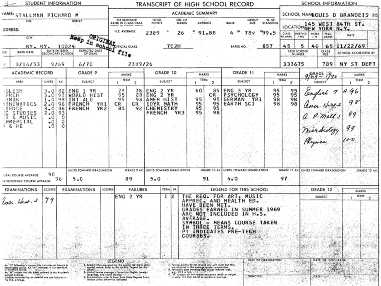
\includegraphics[width=\textwidth]{transcript}
  \caption{\ifdefined\eng Stallman's senior-year transcript at Louis D. Brandeis H.S., November, 1969. Note turnaround in English class performance. ``He was forced to kowtow to a certain degree,'' says his mother, ``but he did it.''\fi\ifdefined\chs 到了1969年11月,当斯托曼即将从布兰德斯高中毕业时,他的英语成绩已经相当出色了。李普曼回忆说:``他虽然很不情愿写作文,但他还是出色地完成了学业。''\fi}
\end{figure}
\fi

\ifdefined\eng
Outside the classroom, Stallman pursued his studies with even more diligence, rushing off to fulfill his laboratory-assistant duties at Rockefeller University during the week and dodging the Vietnam protesters on his way to Saturday school at Columbia. It was there, while the rest of the Science Honors Program students sat around discussing their college choices, that Stallman finally took a moment to participate in the preclass bull session.
\fi

\ifdefined\chs
学校以外的活动里,斯托曼表现得更加勤奋。每周他都会去洛克菲勒大学完成实验员的工作;周六则一路避开反越南战争抗议者的队伍,去哥伦比亚大学参加科学之星计划的学习班。终于又有机会,科学之星计划的学生凑在一起,聊起未来将去哪所大学。
\fi

\ifdefined\eng
Recalls Breidbart, ``Most of the students were going to Harvard and MIT, of course, but you had a few going to other Ivy League schools. As the conversation circled the room, it became apparent that Richard hadn't said anything yet. I don't know who it was, but somebody got up the courage to ask him what he planned to do.''
\fi

\ifdefined\chs
布莱德巴特回忆:``绝大部分学生都会去哈佛或者麻省理工学院。当然也有人去其他几所常春藤学校。大家聊着说着,斯托曼始终没说话。这时候有个人跳出来,问斯托曼究竟去哪所大学。''
\fi

\ifdefined\eng
Thirty years later, Breidbart remembers the moment clearly. As soon as Stallman broke the news that he, too, would be attending Harvard University in the fall, an awkward silence filled the room. Almost as if on cue, the corners of Stallman's mouth slowly turned upward into a self-satisfied smile.
\fi

\ifdefined\chs
三十多年过去了,布莱德巴特依旧清晰地记得那一刻。``哈佛大学''几个字从斯托曼口中一出,人群一时没了声音。一切都好像事先排练好的一样,坐在角落中的斯托曼露出了一丝微笑。
\fi

\ifdefined\eng
Says Breidbart, ``It was his silent way of saying, `That's right. You haven't got rid of me yet.'\hspace{0.01in}''
\fi

\ifdefined\chs
布莱德巴特说:``那微笑好像在说,`没错,你们还没把我甩开呢。'\hspace{0.01in}''
\fi

\theendnotes
\setcounter{endnote}{0}
